\documentclass{standalone}
\usepackage{tikz}
\usetikzlibrary{automata, positioning, arrows}

\begin{document}
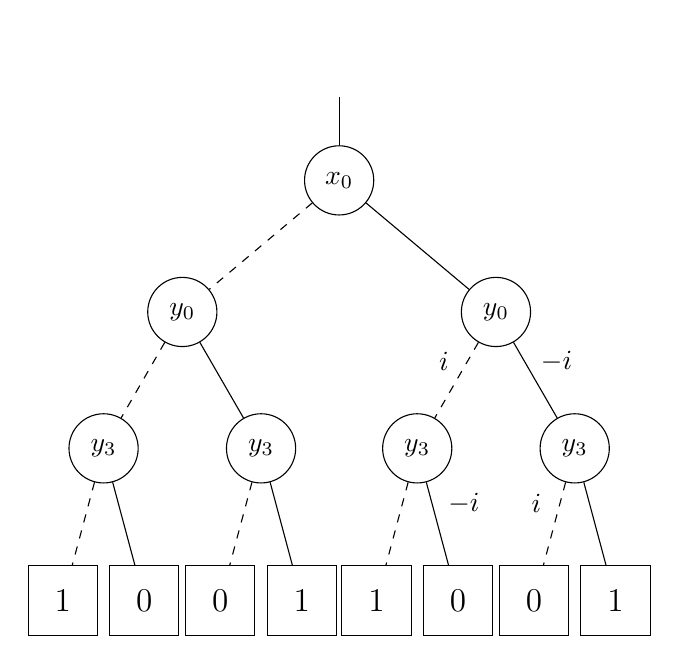
\begin{tikzpicture}[auto,node distance=1.5cm,every node/.style={shape=circle , align=center,solid,minimum size =0.01cm}]
  \tikzstyle{every state}=[fill=white,draw=black,text=black]

  \node[state] (A) {$x_0$};
  \node[state] (B) at ([shift = ({220:2.6cm})]A) {$y_0$};
  \node[state] (C) at ([shift = ({-40:2.6cm})]A) {$y_0$};
  \node[state] (D) at ([shift = ({240:2cm})]B) {$y_3$};
  \node[state] (E) at ([shift = ({-60:2cm})]B) {$y_3$};
  \node[state] (F) at ([shift = ({240:2cm})]C) {$y_3$};
  \node[state] (G) at ([shift = ({-60:2cm})]C) {$y_3$};
  \node[state,shape = rectangle] (D0) at ([shift = ({-105:2cm})]D) {\large$1$};
  \node[state,shape = rectangle] (D1) at ([shift = ({-75:2cm})]D) {\large$0$};
  \node[state,shape = rectangle] (E0) at ([shift = ({-105:2cm})]E) {\large$0$};
  \node[state,shape = rectangle] (E1) at ([shift = ({-75:2cm})]E) {\large$1$};
  \node[state,shape = rectangle] (F0) at ([shift = ({-105:2cm})]F) {\large$1$};
  \node[state,shape = rectangle] (F1) at ([shift = ({-75:2cm})]F) {\large$0$};
  \node[state,shape = rectangle] (G0) at ([shift = ({-105:2cm})]G) {\large$0$};
  \node[state,shape = rectangle] (G1) at ([shift = ({-75:2cm})]G) {\large$1$};
  \node[state,draw=none] (I) [above of= A]       {};

  \path[-]
  (A) edge[dashed]  node {} (B)
  (A) edge  node {} (C)
  (B) edge[dashed]  node {} (D)
  (B) edge  node {} (E)
  (C) edge[dashed]  node [near start,left] {$i$} (F)
  (C) edge  node [near start,right] {$-i$} (G)
  (D) edge[dashed] node {} (D0)
  (D) edge node {} (D1)
  (E) edge[dashed] node {} (E0)
  (E) edge node {} (E1)
  (F) edge[dashed] node {} (F0)
  (F) edge node [near start,right] {$-i$} (F1)
  (G) edge[dashed] node[near start,left] {$i$} (G0)
  (G) edge node {} (G1)
  (I) edge node{} (A);

\end{tikzpicture}
\end{document}